\documentclass[english,floatsintext,man]{apa6}

\usepackage{amssymb,amsmath}
\usepackage{ifxetex,ifluatex}
\usepackage{fixltx2e} % provides \textsubscript
\ifnum 0\ifxetex 1\fi\ifluatex 1\fi=0 % if pdftex
  \usepackage[T1]{fontenc}
  \usepackage[utf8]{inputenc}
\else % if luatex or xelatex
  \ifxetex
    \usepackage{mathspec}
    \usepackage{xltxtra,xunicode}
  \else
    \usepackage{fontspec}
  \fi
  \defaultfontfeatures{Mapping=tex-text,Scale=MatchLowercase}
  \newcommand{\euro}{€}
\fi
% use upquote if available, for straight quotes in verbatim environments
\IfFileExists{upquote.sty}{\usepackage{upquote}}{}
% use microtype if available
\IfFileExists{microtype.sty}{\usepackage{microtype}}{}

% Table formatting
\usepackage{longtable, booktabs}
\usepackage{lscape}
% \usepackage[counterclockwise]{rotating}   % Landscape page setup for large tables
\usepackage{multirow}		% Table styling
\usepackage{tabularx}		% Control Column width
\usepackage[flushleft]{threeparttable}	% Allows for three part tables with a specified notes section
\usepackage{threeparttablex}            % Lets threeparttable work with longtable

% Create new environments so endfloat can handle them
% \newenvironment{ltable}
%   {\begin{landscape}\begin{center}\begin{threeparttable}}
%   {\end{threeparttable}\end{center}\end{landscape}}

\newenvironment{lltable}
  {\begin{landscape}\begin{center}\begin{ThreePartTable}}
  {\end{ThreePartTable}\end{center}\end{landscape}}




% The following enables adjusting longtable caption width to table width
% Solution found at http://golatex.de/longtable-mit-caption-so-breit-wie-die-tabelle-t15767.html
\makeatletter
\newcommand\LastLTentrywidth{1em}
\newlength\longtablewidth
\setlength{\longtablewidth}{1in}
\newcommand\getlongtablewidth{%
 \begingroup
  \ifcsname LT@\roman{LT@tables}\endcsname
  \global\longtablewidth=0pt
  \renewcommand\LT@entry[2]{\global\advance\longtablewidth by ##2\relax\gdef\LastLTentrywidth{##2}}%
  \@nameuse{LT@\roman{LT@tables}}%
  \fi
\endgroup}


  \usepackage{graphicx}
  \makeatletter
  \def\maxwidth{\ifdim\Gin@nat@width>\linewidth\linewidth\else\Gin@nat@width\fi}
  \def\maxheight{\ifdim\Gin@nat@height>\textheight\textheight\else\Gin@nat@height\fi}
  \makeatother
  % Scale images if necessary, so that they will not overflow the page
  % margins by default, and it is still possible to overwrite the defaults
  % using explicit options in \includegraphics[width, height, ...]{}
  \setkeys{Gin}{width=\maxwidth,height=\maxheight,keepaspectratio}
\ifxetex
  \usepackage[setpagesize=false, % page size defined by xetex
              unicode=false, % unicode breaks when used with xetex
              xetex]{hyperref}
\else
  \usepackage[unicode=true]{hyperref}
\fi
\hypersetup{breaklinks=true,
            pdfauthor={},
            pdftitle={The Search for a Bridge: Idiographic Personality Networks},
            colorlinks=true,
            citecolor=blue,
            urlcolor=blue,
            linkcolor=black,
            pdfborder={0 0 0}}
\urlstyle{same}  % don't use monospace font for urls

\setlength{\parindent}{0pt}
%\setlength{\parskip}{0pt plus 0pt minus 0pt}

\setlength{\emergencystretch}{3em}  % prevent overfull lines

\ifxetex
  \usepackage{polyglossia}
  \setmainlanguage{}
\else
  \usepackage[english]{babel}
\fi

% Manuscript styling
\captionsetup{font=singlespacing,justification=justified}
\usepackage{csquotes}
\usepackage{upgreek}



\usepackage{tikz} % Variable definition to generate author note

% fix for \tightlist problem in pandoc 1.14
\providecommand{\tightlist}{%
  \setlength{\itemsep}{0pt}\setlength{\parskip}{0pt}}

% Essential manuscript parts
  \title{The Search for a Bridge: Idiographic Personality Networks}

  \shorttitle{Idiographic Personality Networks}


  \author{Emorie D Beck\textsuperscript{1}~\& Joshua J Jackson\textsuperscript{1}}

  \def\affdep{{"", ""}}%
  \def\affcity{{"", ""}}%

  \affiliation{
    \vspace{0.5cm}
          \textsuperscript{1} Washington University in St.~Louis  }

  \authornote{
    \newcounter{author}
    Emorie D Beck, Department of Psychological and Brain Sciences,
    Washington University in St.~Louis; Joshua J Jackson, Department of
    Psychological and Brain Sciences, Washington University in St.~Louis.

                      Correspondence concerning this article should be addressed to Emorie D Beck, 1 Brookings St., St.~Louis, MO 63130. E-mail: \href{mailto:edbeck@wustl.edu}{\nolinkurl{edbeck@wustl.edu}}
                          }


  \abstract{Baumert and colleagues call for the use of research on intraindividual
personality processes to understand personality structure and
development but do not provide a clear path forward. We argue that
research using idiographic personality networks represent one avenue of
integration of research on personality processes, structure, and
development. Idiographic networks conceive of personality as unique
combinations of relationships between psychological processes, including
behaviors, emotions, motivation, and affect. To demonstrate, we provide
a brief example of the utility of idiographic personality networks in
research on personality processes, structure, and development.}
  \keywords{personality, networks, structure, processes, development \\

    
  }





\usepackage{amsthm}
\newtheorem{theorem}{Theorem}
\newtheorem{lemma}{Lemma}
\theoremstyle{definition}
\newtheorem{definition}{Definition}
\newtheorem{corollary}{Corollary}
\newtheorem{proposition}{Proposition}
\theoremstyle{definition}
\newtheorem{example}{Example}
\theoremstyle{remark}
\newtheorem*{remark}{Remark}
\begin{document}

\maketitle

\setcounter{secnumdepth}{0}



We agree with the authors that the future of personality science is the
integration of research on personality structure, processes, and
development. However, we found their discussion on how this can be
achieved was frustratingly vague. Specifically, although the authors
discussed the costs of aggregation across different levels of Cattell's
data box and the importance of intraindividual processes in
understanding personality structure and development, they offered few
specific ways for how to move such intraindividual research forward. We
believe that the future of such research lies within an idiographic --
person centered -- framework. There have been many calls for increased
research in intraindividual personality processes (Cervone, 2005;
Molenaar, 2004), as well as agreement that the identification of these
patterns cannot be captured using simple interindividual designs.
However, how to select \emph{what} is measured, how often (\emph{when})
to measure it, \emph{where} to measure it, and \emph{how} to model it
once data are collected are often not discussed.

We feel that idiographic approaches to personality assessment can
facilitate the integration of structure, process, and development. The
current article only hinted at these techniques, which we remedy this by
providing a brief example on how idiographic analysis can inform studies
of intraindividual processes. We argue that such an approach allows for
minimal aggregation of the data box while retaining a degree of
parsimony and conclude with the implications of idiographic techniques
in the study of personality processes, structure, and development.

Idiographic personality networks provide a way to assess how personality
variables are related to one another within a person. Consider the
personality networks in Figure 1 for two subjects, assessed at two time
points across two years.\footnote{The idiographic personality networks
  were constructed using the procedure outlined in Wild et al. (2010).
  For a more detailed description, see Beck and Jackson (2017a). R code
  for constructing these networks are available on the first author's
  GitHub.} Each network is built using Experience Sampling (ESM; Larson
\& Csikszentmihalyi, 1983) data collected on a single individual across
a two-week period. Network nodes represent self-reported behavioral,
emotional, motivational, and situational states. The colored nodes are
personality items, while the white nodes are other emotional,
motivational, or situational states. The edges (or paths) between nodes
are regularized partial contemporaneous correlations (Epskamp, Waldorp,
Mõttus, \& Borsboom, 2016; Wild et al., 2010), which signify concurrent
patterns in the participants' responses -- the tendency for states to
occur together. Together, this means that each network aggregates across
occasions and time but not behaviors or people.

\begin{figure}[htbp]
\centering
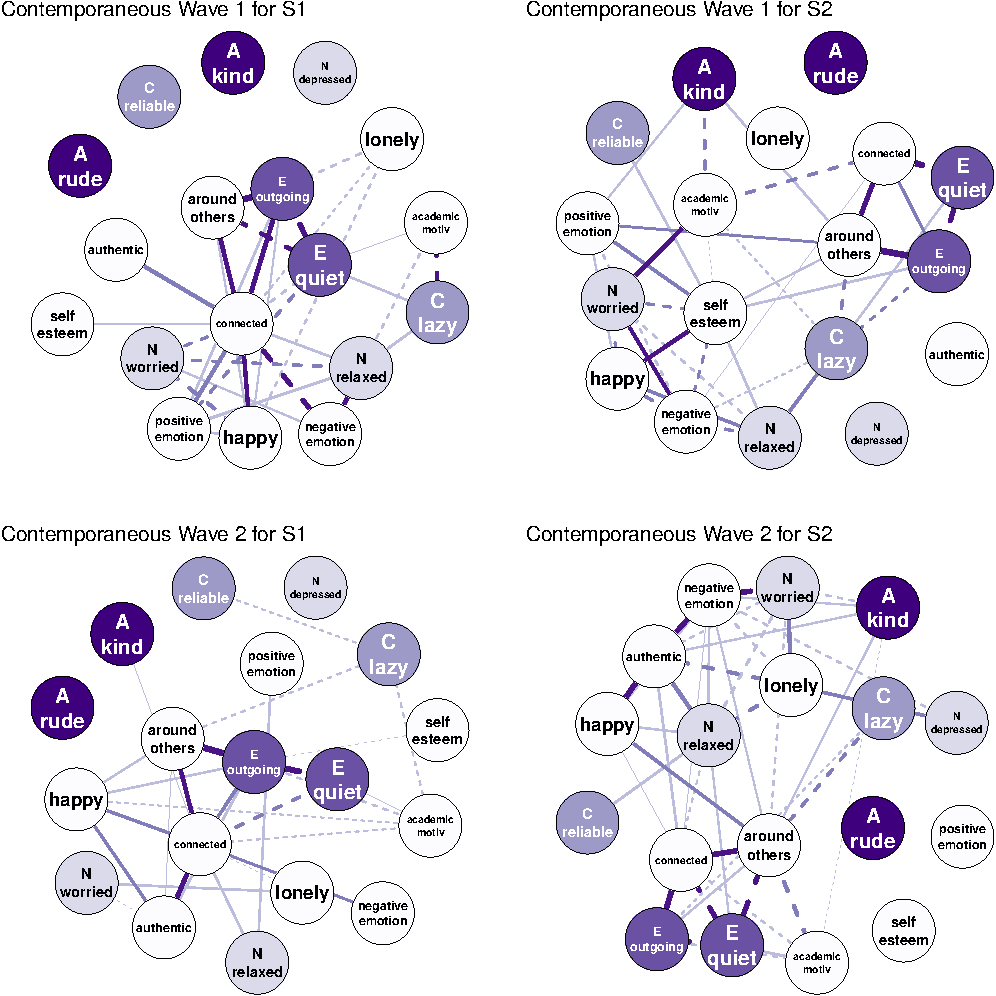
\includegraphics{BeckJacksonFinal_files/figure-latex/unnamed-chunk-4-1.pdf}
\caption{\label{fig:unnamed-chunk-4}Contemporaneous personality networks for
two subjects' ESM responses collected one year apart. The colored nodes
represent personality items, while the white nodes represent behavioral,
emotional, and motivational states. Positive associations (edges) are
solid lines, while negative associations are dashed lines.}
\end{figure}

What can idiographic networks say about personality processes? First,
these networks provide a direct indicator of correspondences between
behaviors and underlying mechanisms (Epskamp et al., 2016). For example,
in Subject 1's personality network, we see strong associations between
feelings of connection to others and other states, including emotions
(e.g. \enquote{happy}), behaviors (e.g. \enquote{outgoing}), and
motivations (e.g. \enquote{around others}). Second, networks highlight
interindividual differences in intraindividual personality structure.
Subject 2's motivation to work on academics repels feelings of
connectedness to others, while Subject 1's network suggests no such
tension. Thus, Subject 2 may struggle to balance academic and social
commitments. Subject 1's academic motivation is related only to being
more quiet and relaxed, while Subject 2's academic motivation is related
to increased worry and decreased kind.ness This opens up new sets of
questions: are specific motivational-behavioral links related to
positive or negative outcomes? Does the relationship between
psychological states change when in different situations (e.g.~academic)
for different people?

For personality structure, idiographic networks underscore how
interindividual differences in intraindividual personality structure may
explain interindividual structure. Comparing the congruence of
idiographic networks with a population network model reproduces a
well-known observation: population models may have little bearing on the
individual (i.e.~not all people evidence a Big 5 structure). In our
sample, congruence between idiographic networks and the population
network was sizeable (\(M = 0.54\)). For wave 1, Subjects 1
(\(r = 0.61\)) and 2 (\(r = 0.64\)) in Figure 1 both exhibit strong
congruence, but there are also considerable individual differences in
congruence across all of our sample (\(SD = 0.26\), range \(-0.28\) to
\(0.81\)). Together, such interindividual differences in intraindividual
personality structure evidence what Baumert and colleagues termed
\enquote{weak emergence} -- macroscopic patterns that emerge out of
microscopic processes. But there are substantial individual differences
in idiographic structure, which opens new avenues for exploration. Who
are the people who fit the population model well and who are those that
do not?

For personality development, personality networks can track changes in
intraindividual personality structure that may not be picked up by
typical nomothetic measures of personality (c.f. Beck \& Jackson,
2017b). For example, both Subject's profiles of ESM composite scores
were stable over 2 years (\(r_{S1} = 0.75\); \(r_{S2} = 0.65\)), but
only Subject 1's personality network (\(r_{S1} = 0.66\);
\(r_{S2} = 0.32\)) was stable over the same time period -- that is,
Subject 1's (but not Subject 2's) stability was reflected both in the
network and the aggregate of their behavior. This observation generates
new questions about the processes of development. What differentiates
people with different patterns of behavioral and network stability?
These findings index changes in the relationship among variables, a type
of change that is rarely explored in personality development (see Beck,
Jackson, and Condon (2017) for an exception).

In sum, we agree with Baumert and colleagues that networks are valuable
tools for personality scientists, perhaps particularly in the generation
of hypotheses in the empirical study of personality processes,
structure, and development. Moreover, we agree that there is opportunity
to examine these three pillars of research simultaneously. A network
perspective personality does not mean throwing out decades of
personality research on nomothetic approaches but does mean reframing
the language we use to talk about personality traits as well as the
explanations of why they occur. We challenge personality researchers to
go beyond Baumert and colleagues' theoretical review and implement
designs capable of tackling personality structure, processes, and
development simultaneously.

\newpage

\section{References}\label{references}

\setlength{\parindent}{-0.5in} \setlength{\leftskip}{0.5in}

\hypertarget{refs}{}
\hypertarget{ref-BeckJackson}{}
Beck, E. D., \& Jackson, J. J. (2017a). A tale of two stabilities: A
longitudinal ESM study of dynamic personality networks. in prep.

\hypertarget{ref-BeckJacksonCorrChange}{}
Beck, E. D., \& Jackson, J. J. (2017b). Do changes in personality imply
changes in behavior? A longitudinal ESM study. in prep.

\hypertarget{ref-BeckJacksonCondonFull}{}
Beck, E. D., Jackson, J. J., \& Condon, D. M. (2017). Personality
network development from 14 to 80. in prep.

\hypertarget{ref-cervone_2005}{}
Cervone, D. (2005). Personality architecture: Within-person structures
and processes. \emph{Annu. Rev. Psychol.}, \emph{56}, 423--452.

\hypertarget{ref-epskamp_2017}{}
Epskamp, S., Waldorp, L. J., Mõttus, R., \& Borsboom, D. (2016).
Discovering psychological dynamics: The gaussian graphical model in
cross-sectional and time-series data. \emph{ArXiv Preprint
ArXiv:1609.04156}.

\hypertarget{ref-larson1983experience}{}
Larson, R., \& Csikszentmihalyi, M. (1983). The experience sampling
method. \emph{New Directions for Methodology of Social \& Behavioral
Science}.

\hypertarget{ref-molenaar_2004}{}
Molenaar, P. C. (2004). A manifesto on psychology as idiographic
science: Bringing the person back into scientific psychology, this time
forever. \emph{Measurement}, \emph{2}(4), 201--218.

\hypertarget{ref-wild_2010}{}
Wild, B., Eichler, M., Friederich, H.-C., Hartmann, M., Zipfel, S., \&
Herzog, W. (2010). A graphical vector autoregressive modelling approach
to the analysis of electronic diary data. \emph{BMC Medical Research
Methodology}, \emph{10}(1), 1.






\end{document}
